{二叉树的遍历方式有{先序遍历、中序遍历、后序遍历和层次遍历}。}

{识记:这里的``先''、``中''、``后''指的都是根结点。}

{\textbf{1. 先序遍历}}

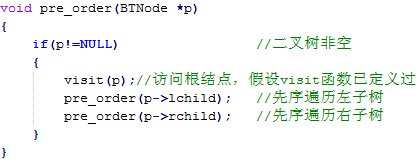
\includegraphics[width=3.70833in,height=1.42708in]{png-jpeg-pics/E4B93F3652A5B6AEA48E90F5E7B51671.png}

{\textbf{2. 中序遍历}}{}{}

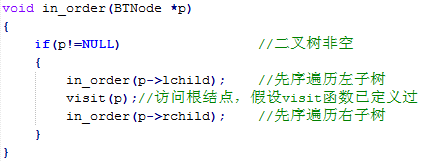
\includegraphics[width=3.70833in,height=1.40625in]{png-jpeg-pics/AA7041D42D263BEB9BB27E2D52669F00.png}

{\textbf{3. 后序遍历}\\
}

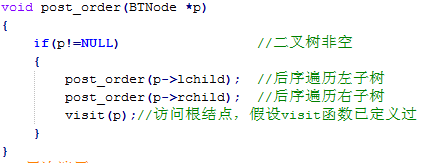
\includegraphics[width=3.70833in,height=1.42708in]{png-jpeg-pics/DA6263531CC4AB6CAFCB3A75F5C3FC2A.png}

{\textbf{4. 层次遍历}}

{设二叉树的根结点所在层数为1,层序遍历就是从所在二叉树的根结点出发,首先访问第一层的树根结点,然后从左到右访问第2层上的结点,接着是第三层的结点,以此类推,{自上而下,自左至右逐层访问树的结点的过程就是层序遍历}。}

{要进行层次遍历需要建立{循环队列}。先将二叉树头结点入队列,然后出队列,访问该结点,如果它有左子树,便将左子树根结点入队,如果它有右子树,便将右子树根结点入队。然后出队列,对出队结点访问,如此反复,直到队列为空为止。}

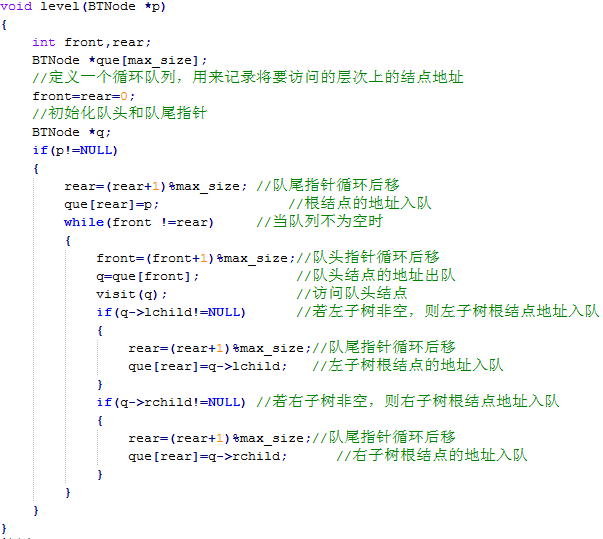
\includegraphics[width=3.70833in,height=3.31250in]{png-jpeg-pics/324D9D425551BAABF5F198A0DB78E7A4.png}

{\textbf{扩展:}}

{\textbf{1. 求二叉树的深度,二叉树以二叉链表为存储方式}}

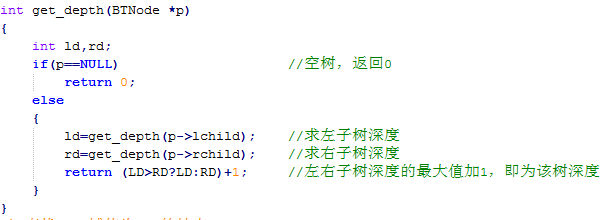
\includegraphics[width=3.70833in,height=1.35417in]{png-jpeg-pics/02C244175A0D32E13628EE7D835406E2.png}

{\textbf{2. 查找data域值为key的结点}\\
}

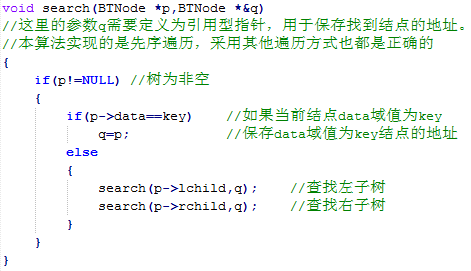
\includegraphics[width=3.70833in,height=2.13542in]{png-jpeg-pics/72561B081410F70646D1B7424340C60D.png}
